\section{Описание интерфейса}

\subsection{Главное окно приложения}
\begin{figure}[h]
	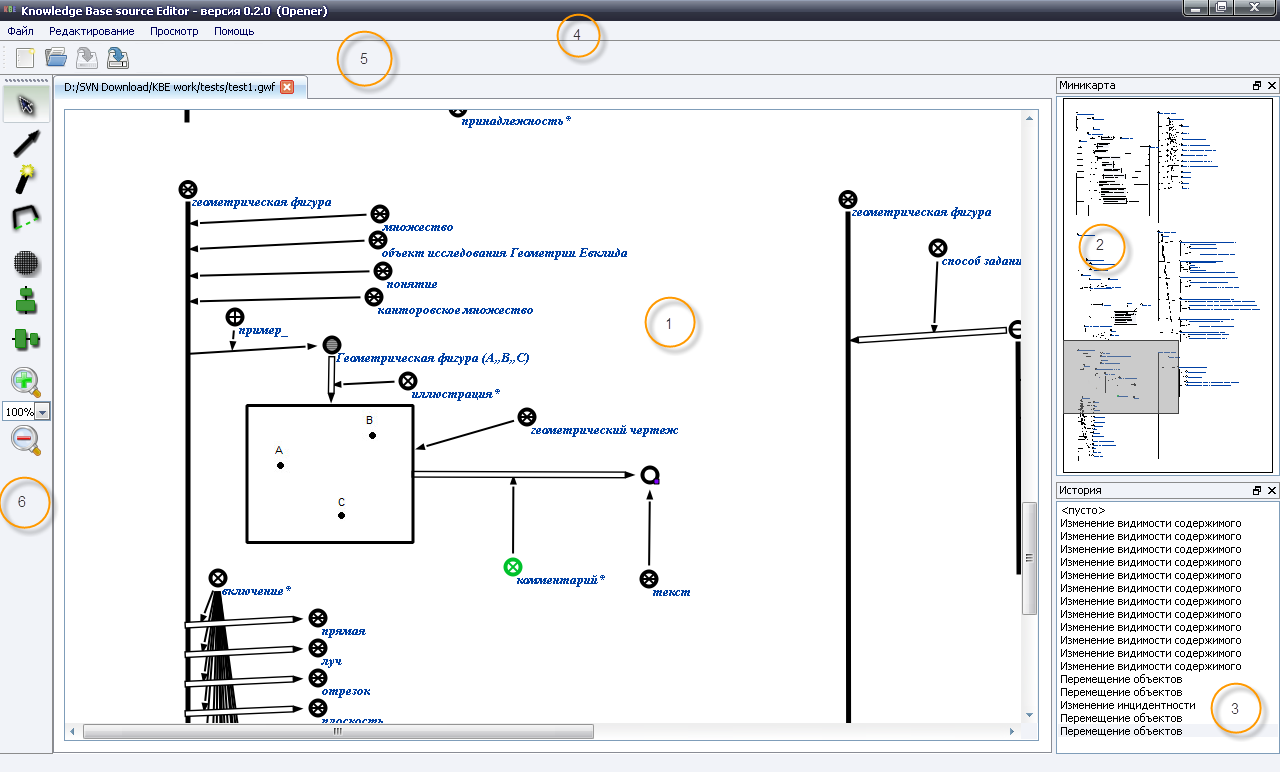
\includegraphics[width=16.23cm, height=9.82cm]{../images/mainwindow.png}
	\caption{Главное окно приложения. 1 – основная рабочая область; 2 – миникарта; 3 – история внесенных в открытый документ 				изменений; 4 – строка меню; 5 – главная панель инструментов; 6 – панель sc.g-инструментов.}
	\label{mainwindow}
\end{figure}
Главное окно приложения представляет собой некоторый набор вкладок и инструментов, которые легко можно перемещать, создавая свою собственную компоновку.

\subsubsection{Основная рабочая область}

Основная рабочая область предоставляет пользователю пространство, состоящее из нескольких вкладок, количество которых соответствует количеству открытых на текущий момент документов. Каждая вкладка является фрагментом исходных текстов базы знаний представленном на некотором внешнем языке. Описание основных действий с объектами рабочей области см. в разделе~\ref{usage}.

\subsubsection{Миникарта и История изменений}

Миникарта предназначена для легкой и быстрой навигации по открытому документу. История внесенных изменений позволяет пользователю отменять и возвращать действия, которые он произвел в ходе редактирования документа.

\hrule\smallskip
\noindent
\includegraphics[width=25pt, height=25pt]{../images/lamp.png} \textcolor[rgb]{.25, .67, .2}{\textbf{Примечание}: Если после отмены группы операций произвести какое либо действие, связанное с редактированием, то отмененные операции будут утеряны.}
\smallskip
\hrule

\subsubsection{Строка меню}

Строка меню содержит основные команды для работы с приложением.
\begin{figure}[h]
	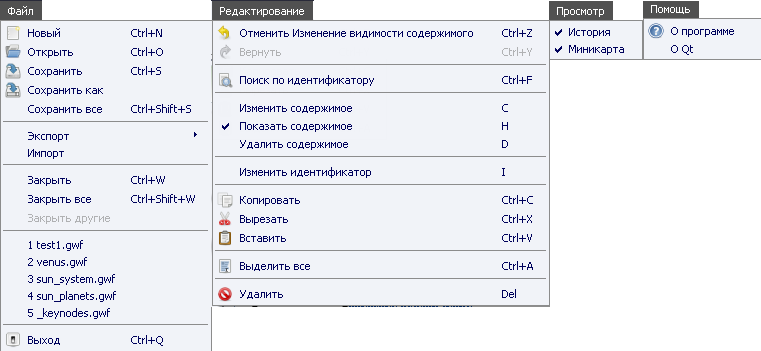
\includegraphics[width=16.22cm, height=7.51cm]{../images/menus.png}
	\caption{Основные меню приложения.}
	\label{menus}
\end{figure}

\hrule
\smallskip
\noindent
\includegraphics[width=25pt, height=25pt]{../images/lamp.png} \textcolor[rgb]{.25, .67, .2}{\textbf{Примечание}: Меню “\textbf{Редактирование}” будет содержать действия в зависимости от выделенных на данный момент объектов. Также оно частично дублируется контекстным меню объекта (открывается по нажатию правой клавищи мыши на объекте).}
\smallskip
\hrule

\subsubsection{Главная панель инструментов}
Содержит основные операции, необходимые для изменения состояния документа.
\begin{figure}[h]
	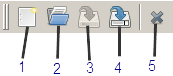
\includegraphics[width=5.72cm, height=2.57cm]{../images/maintoolbar.png}
	\caption{Главная панель инструментов. 1 – создание нового документа; 2 – открытие уже существующего документа; 3 – сохранить 		текущий документ; 4 – сохранить текущий документ как…; 5 - закрыть текущую вкладку .}
	\label{maintoolbar}
\end{figure}